\documentclass[../NormeDiProgetto.tex]{subfiles}
\begin{document}
	\section{Processi di supporto}
		\subsection{Documentazione}
			\subsubsection{Descrizione}
				Di seguito sono riportate le regole che si dovranno seguire per la scrittura
				dei documenti.
			\subsubsection{Approvazione dei documenti}
				Ogni documento deve seguire le seguenti fasi:
				\begin{itemize}
					\item Il documento viene redatto dai vari redattori;
					\item I \verificatori\ procedono al controllo di eventuali errori o
					imprecisioni;
					\item in caso di errori i \verificatori\ procedono a segnalarli ai redattori
					i quali provvedono a correggere gli errori ripartendo dalla prima fase;
					\item Se il documento passa la fase di verifica viene consegnato al
					\responsabilediprogetto\ che decide se approvarlo o meno.\\
					Nel caso venga rifiutato il \responsabilediprogetto\ deve indicare le
					criticità ai redattori i quali provvedono a correggere gli errori
					ripartendo dalla prima fase.
				\end{itemize}
			\subsubsection{Stesura dei documenti}
					Qualora fosse necessario stendere un documento contenente sezioni di testo dove lo stile
					di stesura (frasi, soggetti, verbi, ecc.) andrebbe uniformato ma ci sono più redattori
					all'opera, è necessario fissarne uno comune in modo tale da ottimizzare il lavoro.
					Le decisioni sullo stile di stesura saranno prese all'interno del gruppo attraverso
					gli strumenti di comunicazione adottati oppure riunioni.
				\paragraph{Norme di codifica \LaTeX \\}
					Tutti i file di documentazione devono avere la seguente intestazione:\\
					\\
					\% Document-Author: KaleidosCode\\
					\% Document-Date: GG/MM/AAAA\\
					\% Document-Description: Descrizione documento\\
					\\
					indicando data di creazione e breve descrizione del documento.\\
					Per permettere una migliore lettura del codice \LaTeX, lo stile di indentazione da
					adottare per la stesura dei file di documentazione prevede di indentare il contenuto
					con una tabulazione ogni qualvolta si scriva un nuovo elemento di testo: sezione,
					sottosezione, sotto-sottosezione, paragrafo, ecc.\\
			\subsubsection{Struttura dei documenti}
				\paragraph{Prima pagina\\}
					La prima pagina di ogni documento riporta i seguenti campi:
					\begin{itemize}
						\item Nome dell'università;
						\item Nome del gruppo;
						\item Nome del progetto;
						\item Descrizione del progetto;
						\item Titolo documento con versione;
						\item Logo del gruppo;
						\item Versione;
						\item Data redazione;
						\item Cognome e nome dei redattori del documento;
						\item Cognome e nome dei \verificatori\ del documento;
						\item Cognome e nome del \responsabilediprogetto\ del documento;
						\item Uso;
						\item Lista di distribuzione;
						\item Versione del documento;
						\item E-mail del gruppo.
					\end{itemize} 
				\paragraph{Diario delle modifiche\\}
					Subito dopo la prima pagina è presente una tabella che riassume le modifiche
					apportate al documento ordinate in modo decrescente rispetto alla data.
					Per ogni riga viene indicato:
					\begin{itemize}
						\item Versione del documento;
						\item Data della modifica;
						\item Cognome Nome di chi ha apportato la modifica;
						\item Descrizione della modifica.
					\end{itemize}
				\paragraph{Indici\\}
					In ogni documento (verbali esclusi) viene usato un indice per le sezioni e, nel caso siano
					presenti, anche per grafici e figure. L'indice deve essere posizionato dopo il diario
					delle modifiche.
				\paragraph{Struttura generale delle pagine\\}
					Nell'intestazione delle pagine sono presenti:
					\begin{itemize}
						\item Logo del gruppo;
						\item Nome del documento.
					\end{itemize}
					A piè pagina si possono trovare:    
					\begin{itemize}
						\item Nome del gruppo;
						\item Nome del progetto;
						\item Pagina corrente e pagine totali indicate come "Pagina X di Y" dove
						X indica la pagina attuale e Y le pagine totali.
					\end{itemize}
				\paragraph{Templates\\}
					Per rendere omogenea e semplice la stesura dei documenti e stato creato un
					template in \LaTeX\ che rispetta le regole stilistiche riportate in
					questo documento.
					Questo template è reperibile nel \gl{repository} \gl{GitHub} attraverso il path
					"Documentazione/Templates".\\
					È stato creato anche un template per facilitare la stesura dei verbali che si
					trova nella medesima directory sopra descritta.
			\subsubsection{Norme tipografiche}
				In questa sezione vengono descritte le regole di tipografia e ortografia comuni per
				tutti i documenti.
				\paragraph{Punteggiatura}
					\begin{itemize}
						\item \textbf{Parentesi}: il testo racchiuso tra parentesi non deve iniziare
						o finire con spaziature inoltre alla fine non devono essere presenti
						caratteri di punteggiatura;
						\item \textbf{Punteggiatura}: i caratteri di punteggiatura non devono mai
						essere preceduti da spaziatura;
						\item \textbf{Maiuscole}: l'iniziale maiuscola viene usata per il nome del
						team, del progetto, dei documenti, dei ruoli, delle varie fasi di lavoro e
						per le parole Fornitore, Proponente e Committente qualora usate pronominalmente.\\
						Inoltre viene usata negli elenchi puntati e nei casi indicati dalla lingua
						italiana.
					\end{itemize}
				\paragraph{Stile di testo}
					\begin{itemize}
						\item \textbf{Corsivo}: usato nei seguenti casi:
						\begin{itemize}
							\item \textbf{Citazioni}: viene usato il corsivo quando una frase viene
							citata;
							\item \textbf{Abbreviazioni}: viene usato per evidenziare abbreviazioni;  
							\item \textbf{Nomi particolari}: i nomi di figure particolari come
							\textit{Progettista} o \textit{Analista};  
							\item \textbf{Documenti}: viene usato il corsivo per i nomi dei vari
							documenti.
						\end{itemize}
						\item \textbf{Grassetto}: usato nei seguenti casi:
						\begin{itemize}
							\item \textbf{Elenchi puntati}: viene usato il grassetto per parole o
							frasi chiave all'interno di un elenco.
						\end{itemize}			
						viene inoltre usato per parole o particolari passaggi importanti;
						\item \textbf{Maiuscolo}: usato soltanto per acronimi o eventuali macro
						\LaTeX\ nei documenti;
						\item \textbf{\LaTeX }: per ogni riferimento a \LaTeX\ bisogna utilizzare il
						comando \textbackslash LaTeX.
					\end{itemize}
				\paragraph{Composizione del testo}
					\begin{itemize}
						\item \textbf{Elenchi puntati}: prima lettera minuscola (salvo casi
						precedenti) e devono terminare con punto e virgola, tranne l'ultimo elemento
						che terminerà con il punto;
						\item \textbf{Note a piè pagina}: prima lettera maiuscola e devono terminare
						con il punto.
					\end{itemize}
				\paragraph{Formati}
					\begin{itemize}
						\item \textbf{Numeri}: uso dello standard SI/ISO 31-10; 
						\item \textbf{Percorsi}: deve essere usato il comando
						\LaTeX\ \textbackslash url per indirizzi web o mail;
						\item \textbf{Ore}: le ore devono seguire lo standard ISO 8601 quindi
						espresse come:\\
						\begin{center}
							HH:MM 
						\end{center}  
						dove HH indica l'ora espressa con 2 cifre (00-23) e MM indica i minuti
						espressi sempre con 2 cifre (00-59);
						\item \textbf{Date}: le date devono seguire lo standard italiano-europeo
						UNI EN 28601 quindi saranno espresse come:
						\begin{center}
							GG/MM/AAAA
						\end{center}  
						dove GG indica 2 cifre per il giorno, MM indica 2 cifre per il mese e AAAA indica 
						4 cifre per l'anno.
					\end{itemize}
				\paragraph{Riferimenti vari\\}
					Per i vari riferimenti si devono usare i seguenti comandi \LaTeX\ (che
					garantiscono la corretta scrittura, con la prima lettera di ogni parola che non
					sia una preposizione maiuscola):
					\begin{itemize}
						\item \textbf{Ruoli}: per i ruoli si devono usare i seguenti comandi:
						\begin{itemize}
							\item \textbackslash responsabilediprogetto =
							\responsabilediprogetto; 
							\item \textbackslash amministratore = \amministratore;
							\item \textbackslash analista = \analista;
							\item \textbackslash progettista = \progettista;
							\item \textbackslash programmatore = \programmatore;
							\item \textbackslash verificatore = \verificatore;
							\item \textbackslash segretario = \segretario;
							\item \textbackslash amministratori= \amministratori;
							\item \textbackslash analisti = \analisti;
							\item \textbackslash progettisti = \progettisti;
							\item \textbackslash programmatori = \programmatori;
							\item \textbackslash verificatori = \verificatori;
							\item \textbackslash segretari = \segretari.
						\end{itemize}	
						\item \textbf{Documenti}: per i documenti si devono usare i seguenti
						comandi:
						\begin{itemize}
							\item \textbackslash pianodiprogetto = \pianodiprogetto;
							\item \textbackslash pianodiqualifica = \pianodiqualifica;
							\item \textbackslash normediprogetto = \normediprogetto;
							\item \textbackslash studiodifattibilita = \studiodifattibilita;
							\item \textbackslash analisideirequisiti = \analisideirequisiti;
							\item \textbackslash specificatecnica = \specificatecnica;
							\item \textbackslash definizionediprodotto = \definizionediprodotto;
							\item \textbackslash manualeutente = \manualeutente;
							\item \textbackslash glossario = \glossario.
						\end{itemize}	
						\item \textbf{Documenti con versione}: per i documenti con versione si
						devono usare i seguenti comandi:
						\begin{itemize}
							\item \textbackslash pianodiprogettov = \pianodiprogettov;
							\item \textbackslash pianodiqualificav = \pianodiqualificav;
							\item \textbackslash normediprogettov = \normediprogettov;
							\item \textbackslash studiodifattibilitav = \studiodifattibilitav;
							\item \textbackslash analisideirequisitiv = \analisideirequisitiv;
							\item \textbackslash specificatecnicav = \specificatecnicav;
							\item \textbackslash definizionediprodottov = \definizionediprodottov;
							\item \textbackslash manualeutentev = \manualeutentev;
							\item \textbackslash glossariov = \glossariov.
						\end{itemize}	
						\item \textbf{Revisione}: per le revisioni si devono usare i seguenti
						comandi:
						\begin{itemize}
							\item \textbackslash revisionedeirequisiti = \revisionedeirequisiti;
							\item \textbackslash revisionediaccettazione =
							\revisionediaccettazione;
							\item \textbackslash revisionediprogettazione =
							\revisionediprogettazione;
							\item \textbackslash revisionediqualifica = \revisionediqualifica.		
						\end{itemize}
						\item \textbf{Nome del gruppo}: per il nome del gruppo definito come
						``\kaleidoscode '' si dovrà usare \textbackslash kaleidoscode;
						\item \textbf{Nome del Proponente}: per riferirsi al Proponente come
						``\proponente '' si dovrà usare \textbackslash proponente;	
						\item \textbf{Nome del Committente}: per riferirsi al Committente come
						``\vardanega ''  si dovrà usare \textbackslash vardanega;
						\item \textbf{Nome del progetto}: per riferirsi al progetto come
						``\progetto '' si dovrà usare \textbackslash progetto.
					\end{itemize}
					Inoltre i nomi di file senza percorso completo si devono scrivere usando il
					formato monospace e per scrivere nomi dei componenti si deve usare il formato
					"Cognome Nome". 
				\paragraph{Sigle\\}
					Per rendere più accessibili tabelle e diagrammi si devono usare (dove
					necessario) le seguenti sigle:
					\begin{itemize}
						\item \textbf{AdR}: \analisideirequisiti;
						\item \textbf{GL}: \glossario;
						\item \textbf{NdP}: \normediprogetto;
						\item \textbf{PdP}: \pianodiprogetto;
						\item \textbf{PdQ}: \pianodiqualifica;
						\item \textbf{SdF}: \normediprogetto;
						\item \textbf{ST}: \specificatecnica;
						\item \textbf{RA}: \revisionediaccettazione;
						\item \textbf{RP}: \revisionediprogettazione;
						\item \textbf{RQ}: \revisionediqualifica;
						\item \textbf{RR}: \revisionedeirequisiti.
					\end{itemize}
			\subsubsection{Componenti grafiche}
				\paragraph{Tabelle\\}
					Ogni tabella deve essere accompagnata da una descrizione che specifichi anche
					l'indice ad essa associata per renderla tracciabile all'interno del documento.
				\paragraph{Immagini\\}
					Le immagini devono essere convertite in formato png o jpg prima di essere incorporate nei
					documenti e ciascuna deve essere accompagnata da una descrizione che specifichi anche l'indice ad
					essa associata.
			\subsubsection{Classificazione documenti}
				\paragraph{Documenti formali\\}
					Un documento è ritenuto formale solo dopo essere stato approvato dal
					\responsabilediprogetto, dopo l'approvazione viene considerato pronto per la
					revisione da parte del Committente.
				\paragraph{Documenti informali\\}
					Un documento è ritenuto informale fino all'approvazione del
					\responsabilediprogetto, fino a quel momento è considerato ad uso interno.
			\subsubsection{Versionamento}
				Ogni documento deve essere accompagnato dal numero della versione attuale così
				formato:
				\begin{center}
					vX.Y.Z
				\end{center}
				dove:
				\begin{itemize}
					\item \textbf{X}: numero di uscite formali del documento e aumenta ad ogni
					approvazione da parte del \responsabilediprogetto;
					\item \textbf{Y}: usato per modifiche sostanziali e verifiche;
					\item \textbf{Z}: usato per indicare modifiche minori. 
				\end{itemize}
				Per riferirsi a una specifica versione del documento si deve usare il seguente
				formato:
				\begin{center}
					\textit{Nome Documento vX.Y.Z}
				\end{center}
				mentre il nome da applicare ai file è:
				\begin{center}
					NomeDocumento\_vX.Y.Z.pdf
				\end{center}
				\paragraph{Variazione indici\\}
					Le variazioni degli indici avvengono nel seguente modo:
					\begin{itemize}
						\item \textbf{X}: deve essere aggiornata dal \responsabilediprogetto\ dopo
						la sua approvazione;
						\item \textbf{Y}: deve essere incrementato da chi esegue la modifica o la
						verifica;
						\item \textbf{Z}: deve essere incrementato da chi esegue la modifica.
					\end{itemize}
					Queste modifiche sono visibili dal diario delle modifiche.
			\subsubsection{Verbale}
					\paragraph{Riunione interna (\gl{chat}/videoconferenze incluse)\\}
						Il verbale di riunione interna è un documento informale che permette di tenere traccia
						degli argomenti discussi in ogni riunione. Il segretario, scelto a rotazione, ha il
						compito di redigere questo documento. Il verbale prodotto deve poi essere condiviso
						con tutti i membri del gruppo mediante \gl{Google Drive}, in modo da rendere sempre
						disponibile e accessibile il contenuto dello stesso.\\
						Qualora un verbale di riunione interna debba essere fornito in sede di revisione,
						dovrà essere redatto in \LaTeX\ utilizzando il template fornito allo scopo.
					\paragraph{Riunione esterna\\}
						In caso di riunione esterna con il Proponente e/o Committente, il verbale è un
						documento ufficiale che può avere valore normativo e deve quindi essere redatto
						in \LaTeX\ utilizzando il template fornito allo scopo, come già scritto precedentemente.
						Anche questi verbali devono essere condivisi tra i membri del gruppo
						attraverso Google Drive.
					\paragraph{Struttura verbale\\}
						La prima pagina di ogni verbale riporta i seguenti campi:
						\begin{itemize}
							\item Nome dell'università;
							\item Nome del gruppo;
							\item Nome del progetto;
							\item Descrizione del progetto;
							\item Oggetto;
							\item Logo del gruppo;
							\item Data redazione;
							\item Cognome e nome del redattore del documento;
							\item Cognome e nome del \verificatore\ del documento;
							\item Cognome e nome del \responsabilediprogetto\ del documento;
							\item Uso;
							\item Lista di distribuzione;
							\item E-mail del gruppo.
						\end{itemize}
						La pagina successiva deve contenere le informazioni sulla riunione:
						\begin{itemize}
							\item Data riunione;
							\item Luogo dell'incontro;
							\item Ora di inizio;
							\item Ora di fine;
							\item Partecipanti.
						\end{itemize}
						Infine deve essere presente:
						\begin{itemize}
							\item L'ordine del giorno;
							\item Il riassunto delle discussioni fatte.
						\end{itemize}
			\subsubsection{Glossario}
				Il \glossario\ conterrà alcune parole presenti negli altri documenti, che possono essere
				termini generanti ambiguità d'interpretazione oppure far parte del contesto di applicazione.
				I termini sono raggruppati per lettera iniziale e ordinati secondo criterio lessicografico.
				Ogni termine presente nel \glossario\ deve aver associato una descrizione concisa.
				I termini andranno inseriti parallelamente alla stesura degli altri documenti.
		\subsection{Verifica}
			\subsubsection{Scopo del processo}
				Scopo della verifica è quello di accertare che documenti e file di codice prodotti non
				contengano errori e che rispettino le regole riportate in questo documento.
			\subsubsection{Attività}
				Compito dei \verificatori\ è quello di redigere una lista con gli errori più comuni trovati
				durante lo svolgimento della loro attività nella documentazione, che verrà integrata
				progressivamente. Tale lista si trova in appendice a questo documento e serve a
				migliorare i processi di verifica successivi.
				\paragraph{Gestione degli errori trovati in documentazione\\}
					Qualora i \verificatori\ trovassero degli errori all'interno dei documenti devono
					identificare il tipo di errore trovato e agire di conseguenza
					secondo la lista proposta in seguito:
					\begin{itemize}
						\item Errore \textbf{piccolo}: errori ortografici, grammaticali, di stesura delle
						frasi dovranno essere corretti dal \verificatore\ stesso;
						\item Errore \textbf{medio}: errori di organizzazione del documento, di gestione
						dell'indice possono essere corretti dal \verificatore;
						\item Errore \textbf{grave}: errori quali la mancanza di sezioni nel documento o una
						grande disorganizzazione dell'indice e dei contenuti, devono essere segnalati ai
						redattori, attraverso lo strumento di comunicazione \gl{Slack}, i quali devono
						provvedere alla correzione e sistemazione.
					\end{itemize}
				\paragraph{Gestione degli errori trovati nel codice\\}\label{GestioneErroriCodice}
					Per tenere traccia degli errori al codice si deve usare il servizio ``Issues'' messo a
					disposizione da GitHub.\\
					Qualora i \verificatori\ trovassero degli errori all'interno del codice o attraverso il
					test dello stesso, devono seguire la procedura sottostante:
					\begin{itemize}
						\item Il \verificatore\ deve aprire una nuova issue con la descrizione
						del problema;
						\item Il \responsabilediprogetto\ deve verificare questa issue e provvedere ad
						assegnarla ad un programmatore;
						\item Una volta risolta e verificata viene segnata come risolta da parte
						del \responsabilediprogetto.
					\end{itemize}
				\paragraph{Analisi Statica\\}
					Una tecnica di verifica che si applica al codice sorgente e alla documentazione
					e non richiede l'esecuzione del prodotto software.
					Le principali strategie sono due:
					\begin{itemize}
						\item Inspection: questa tecnica si applica quando si conoscono le
						problematiche oggetto di verifica. Consiste in una ricerca mirata attraverso il
						documento per l'identificazione dei problemi, nel caso di documentazione,
						basandosi su una lista di errori precedentemente stilata
						(come scritto sopra, tale lista si trova in appendice).
						\item Walkthrough: questa tecnica consiste nello scorrere l'intero
						documento alla ricerca di errori generici. Viene applicata sopratutto nelle
						prime fasi di stesura del documento o di codifica a causa dell'impegno
						necessario per attuarla, che aumenta notevolmente con l'aumentare delle
						dimensioni del documento da verificare.
					\end{itemize}
					Per eseguire una prima verifica automatica dei documenti, viene usato il controllo
					ortografico	LanguageTool v3.6, integrabile nell'editor \LaTeX\ consigliato, TexStudio.
				\paragraph{Analisi Dinamica\\}
					Questa tecnica può essere applicata solo al software, nella sua interezza o solo
					in parte.
					Consiste nell'usare una serie di test automatici creati dal gruppo che mettano
					alla prova il software prodotto e restituiscano risultati relativi a eventuali
					problemi rilevati.
					I test devono essere ripetibili durante l'intero ciclo di vita e devono coprire
					un insieme finito di casi, con valori di ingresso, uno stato iniziale ed esito
					decidibile.
				\paragraph{Analisi dei rischi\\}
					Il \responsabilediprogetto\ deve monitorare i rischi indicati nel \pianodiprogettov.
					Qualora ne identifichi di nuovi deve:
					\begin{itemize}
						\item Mettere al corrente il team;
						\item Elaborare una nuova strategia per la gestione dei nuovi rischi;
						\item Aggiornare il documento \pianodiprogetto.
					\end{itemize}
		\subsection{Validazione}
			\subsubsection{Scopo del processo}
				La validazione si occupa di accertare che il prodotto realizzato sia conforme
				alle attese.
			\subsubsection{Attività}
				Di questa fase si occupa il \responsabilediprogetto\ il quale deve verificare
				che i documenti e il codice sorgente rispetti a pieno i requisiti imposti dal
				Committente e dal Proponente.\\
				Una volta che i	documenti ottengono l'approvazione dei \verificatori, il
				\responsabilediprogetto\ controlla eventuali errori o mancanze.
				Nel caso se ne identifichino, si devono segnalare le criticità ai
				redattori che provvederanno a correggerle.
		
		\subsection{Strumento di versionamento}\label{StrumentoDiVersionamento}
			Sono stati presi in considerazione diversi software di versionamento (\gl{Git}, SVN, Mercurial)
			prima di decidere di usare \textbf{Git}. I motivi principali della scelta sono: 
			\begin{itemize}
				\item \textbf{Flessibilità}: Git è un repository distribuito con la possibilità di
				\textit{commit} e \textit{revert} locali;
				\item \textbf{Esperienza del team}: Git è già stato usato da alcuni componenti
				del gruppo \kaleidoscode.
			\end{itemize}
			In particolare, si è deciso di utilizzare il servizio di hosting GitHub, vista la richiesta
			del Proponente all'interno del capitolato d'appalto.
			In ogni repository il \gl{branch} ``Master'' deve contenere solamente versioni di documentazione e/o
			codice approvate dal \responsabilediprogetto. Per questo motivo deve essere creato almeno un
			branch alternativo nel quale lavorare liberamente.
			Nel caso di repository contenenti codice, i branch ``Master'' e di sviluppo devono essere
			sottoposti ad analisi statica e dinamica; saranno rigettati se non conformi.
			Qualora più persone debbano lavorare ad uno stesso file, dovranno creare dei nuovi branch ad ogni
			implementazione di una modifica rilevante.
			L'operazione di integrazione continua verrà svolta dallo strumento descritto in sezione
			\ref{IntegrazioneContinua}.
			Al completamento di un incremento, è possibile effettuare una richiesta di \gl{merge}.
			Un \verificatore\ avrà in compito di controllare il merge e di accettarlo oppure di segnalare
			la presenza di eventuali errori come descritto in sezione \ref{GestioneErroriCodice}.
			\subsubsection{Descrizione dei commit}
			La cronologia dei commit sarà utilizzata dal \responsabilediprogetto\ come log per determinare l'effettivo stato di avanzamento del progetto. Ogni commit effettuato dovrà perciò riportare una descrizione chiara e concisa di quanto fatto. Nel titolo del commit si consiglia di usare le seguenti notazioni:
			\begin{itemize}
				\item \textbf{$+$ [nomefile, nomesezione, nomeoggetto]} indica l'aggiunta del file \textit{nomefile}, oppure la stesura della sezione \textit{nomesezione} o in generale la creazione dell'oggetto \textit{nomeoggetto};
				\item \textbf{$-$ [nomefile, nomesezione, nomeoggetto]} indica la rimozione del file \textit{nomefile}, della sezione \textit{nomesezione} o dell'oggetto \textit{nomeoggetto};
				\item \textbf{$\sim$ [nomefile, nomesezione, nomeoggetto]} indica la modifica del file \textit{nomefile}, della sezione \textit{nomesezione} o dell'oggetto \textit{nomeoggetto}. In questo caso è obbligatorio inserire una descrizione più approfondita della modifica effettuata.
			\end{itemize}
		\subsection{Altri strumenti}
			\subsubsection{Google Drive}
			\begin{figure} [h!]
				\centering
				
\includegraphics[scale=0.2]{./Immagini/Drive.png}
				\caption{Schermata di presentazione di Google Drive}\label{}
			\end{figure}
				In questo servizio di condivisione vengono messi solo file che non necessitano di
				controllo di versione.
				Esso conterrà:
				\begin{itemize}
					\item Documenti che sono recuperabili da altre fonti (es. \gl{internet});
					\item File di installazione dei software utilizzati dal gruppo.
					In questo modo si punta a garantire l'uso della stessa versione software per ogni
					componente del gruppo;
					\item I manuali (software, libri, pdf, ...) di consultazione, così da avere
					uniformità di versione e di informazione;
					\item I file pdf dei verbali redatti.
				\end{itemize}
				La possibilità di installare Drive sul proprio PC dà modo ad ogni componente del gruppo di
				avere a disposizione documentazione e software anche offline.
				Google Drive viene utilizzato come strumento di supporto allo sviluppo della
				documentazione e del software presente su Git.
			\subsubsection{ProjectLibre}
			\begin{figure} [h!]
				\centering
				
\includegraphics[scale=0.3]{./Immagini/Libre.png}
				\caption{Logo di ProjectLibre}\label{}
			\end{figure}
				Per pianificare le attività legate allo sviluppo del progetto e la gestione delle risorse
				si è scelto di utilizzare \textbf{ProjectLibre}.
				ProjectLibre è un programma open source per il project management. È basato su Java ed è
				quindi eseguibile su ogni sistema operativo. È il successore ufficiale di OpenProj. Tale
				software è stato scelto in quanto:
				\begin{itemize}
					\item È portabile, essendo basato su Java;
					\item È open-source;
					\item Genera \gl{diagrammi Gantt};
					\item Genera automaticamente diagrammi Program Evaluation and Review Technique (\gl{PERT})
					a partire dal Gantt;
					\item Genera automaticamente la \gl{Work Breakdown Structure} (WBS), a partire dal Gantt
					con allocazione di risorse;
					\item Calcola i parametri \gl{Schedule Variance}(SV) e \gl{Budget Variance} (BV);
					\item Permette il salvataggio su file \gl{XML}: essendo un file testuale è possibile
					fare il merge dei file in caso di conflitti su repository. 
				\end{itemize}
			\subsubsection{\gl{\LaTeX}}
				Per la stesura dei documenti è stato scelto di utilizzare il linguaggio \LaTeX.
				La scelta è stata quasi obbligata in quanto \LaTeX\ permette di separare il contenuto dalla
				formattazione, permettendo un versionamento più semplice e consentendo di definire template condivisi per uniformare i documenti. Altre soluzioni come Microsoft Office, LibreOffice o
				Google Docs non avrebbero consentito un livello altrettanto elevato di separazione portando
				ad un aumento del lavoro da parte dei membri del gruppo e una maggior difficoltà di
				uniformazione dei contenuti.
				Per la scrittura di documenti \LaTeX\ l'editor consigliato è \textbf{TeXstudio}.
			\subsubsection{Strumenti per il controllo ortografico}
				Per eseguire una verifica automatica dei documenti approssimativa,
				viene usato il programma di controllo ortografico LanguageTool versione 3.6, integrabile
				nell'editor \LaTeX\ TexStudio.
			\subsubsection{Strumenti per i diagrammi UML}	
				Per creare i diagrammi UML dei casi d'uso presenti nel documento \analisideirequisitiv,
				è stato scelto di utilizzare Astah, vista la semplice interfaccia e la presenza di una
				versione gratuitamente scaricabile.
				I diagrammi dei casi d'uso sono in gran parte generati automaticamente utilizzando PlantUML.
			\subsubsection{SWEgo}
				Per effettuare il tracciamento dei requisiti è stato scelto di realizzare un'applicazione
				web accessibile attraverso \gl{browser} ed ospitata su un server dedicato: SWEgo.
				Tale applicativo permette di aggiungere casi d'uso, attori partecipanti e requisiti.
				Casi d'uso e requisiti sono automaticamente identificati attraverso i codici auto-generati
				dall'applicazione; È inoltre possibile esportare il codice \LaTeX\ elenca casi d'uso,
				requisiti e le loro relazioni.
				\begin{figure} [h!]
					\centering
					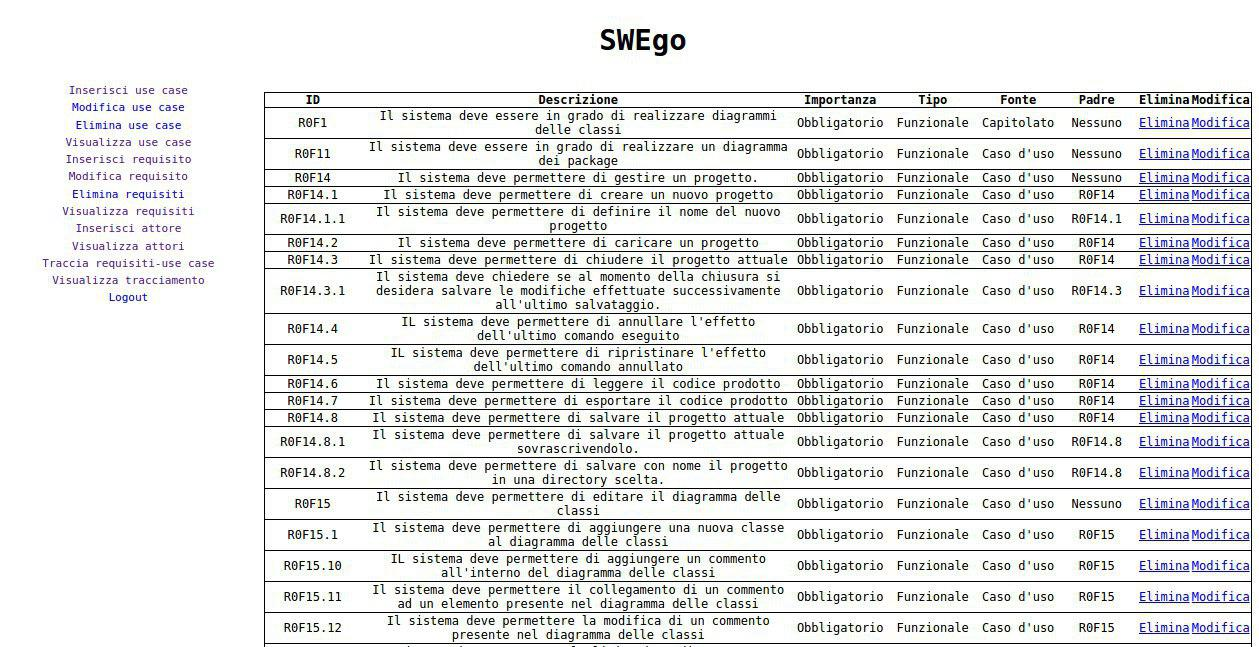
\includegraphics[scale=0.42]{./Immagini/SWEgo.jpg}
					\caption{Schermata di tracciamento requisiti in SWEgo}\label{}
				\end{figure}
			\subsubsection{Strumenti per l'usabilità}
				L'usabilità descritta nel \pianodiqualificav, verrà testata attraverso la prova del prodotto
				ad un piccolo numero di volontari fornendo consigli al gruppo su come effettuare
				miglioramenti principalmente alle interfacce grafiche.\\
				Le persone volontarie dovranno rientrare nella categoria degli utenti target del prodotto
				descritti nell'\analisideirequisitiv.
			\subsubsection{Strumenti per l'integrazione continua}\label{IntegrazioneContinua}
				Per l'operazione di integrazione continua è stato scelto Jenkins.\\
				Tale strumento permette di impostare la compilazione del codice e può essere utilizzato con
				i principali strumenti di gestione del codice sorgente tra cui Git (sezione
				\ref{StrumentoDiVersionamento}).
				La sua esecuzione è azionata ad ogni commit.
				Jenkins sarà utilizzato principalmente nella fase di codifica.
			\subsubsection{Strumenti per la validazione \gl{W3C}}
				L'applicativo web verrà testato anche attraverso gli strumenti di validazione online:
				\begin{itemize}
					\item \url{https://validator.w3.org/} (02/04/2017) per le pagine web;
					\item \url{https://jigsaw.w3.org/css-validator/} (02/04/2017) per i fogli di stile.
				\end{itemize}
			\subsubsection{Script}
				È stato deciso di usare \gl{script} dedicati per le seguenti operazioni:
				\begin{itemize}
					\item Calcolo dell'indice Gulpease, dove uno script dedicato provvede a fornire i valori
					calcolati per i vari documenti.
				\end{itemize}
\end{document}